\begin{figure}[h]
    \centering
    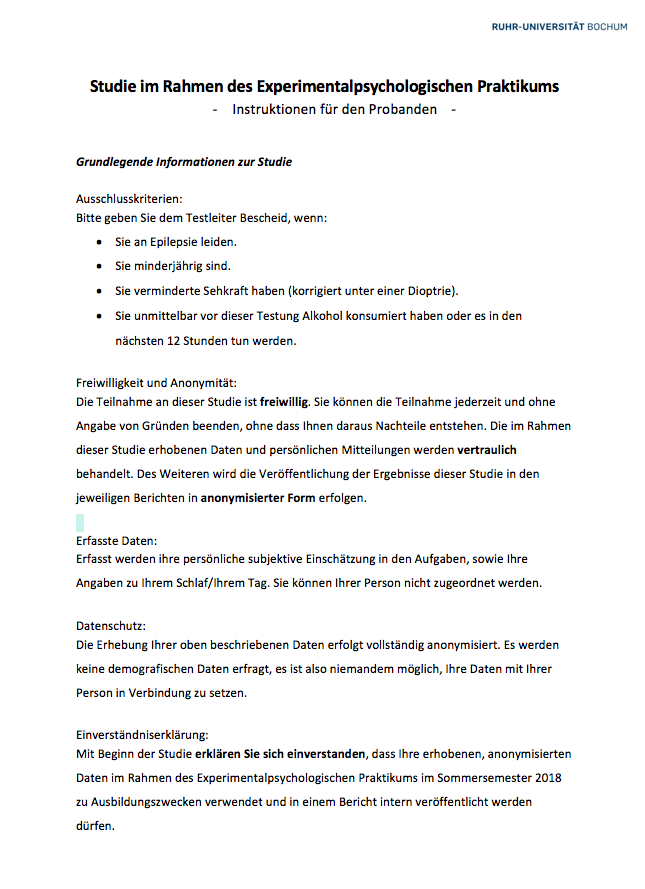
\includegraphics[width=100mm]{Bilder/ProbVOR.png}
    \caption{Instruktion vor der Testung}
\end{figure}
\newpage

%\begin{figure}[h]
    %\centering
    %
\includegraphics[width=90mm]{Bilder/ProbT1.png}
    %\caption{Instruktion zum ersten Messzeitpunkt}
%\end{figure}

%\begin{figure}[h]
    %\centering
    %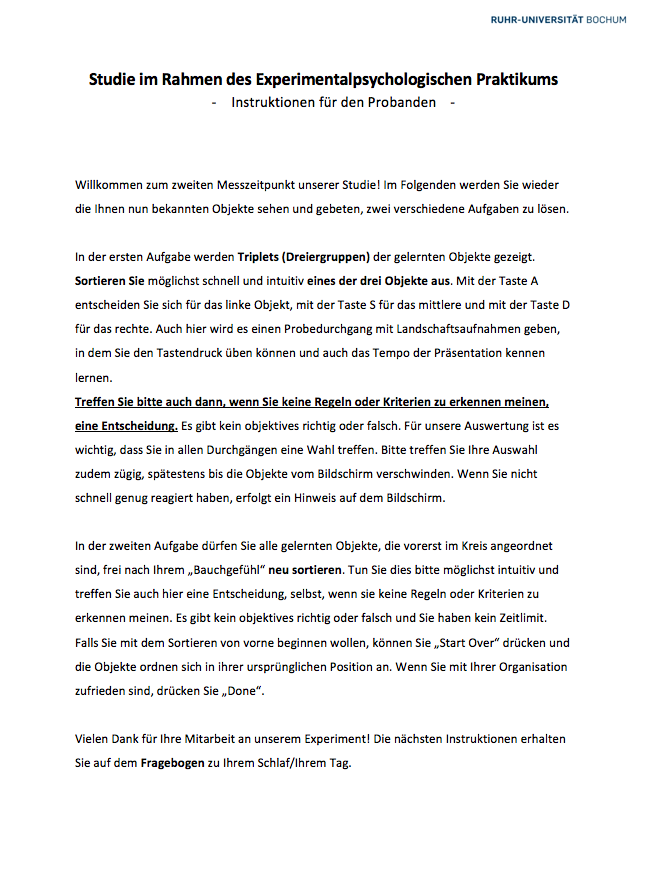
\includegraphics[width=85mm]{Bilder/ProbT2.png}
    %\caption{Instruktion zum zweiten Messzeitpunkt}
%\end{figure}

\begin{figure}[H]
  \centering
  \captionsetup[subfigure]{labelformat=empty}
  \setkeys{Gin}{width=66mm,keepaspectratio}%
  \vspace{0.5 cm}
  \subfloat[Instruktion Messzeitpunkt 1]{
\includegraphics{Bilder/ProbT1.png}} 
  \hspace{0.5cm}
  \subfloat[Instruktion Messzeitpunkt 2]{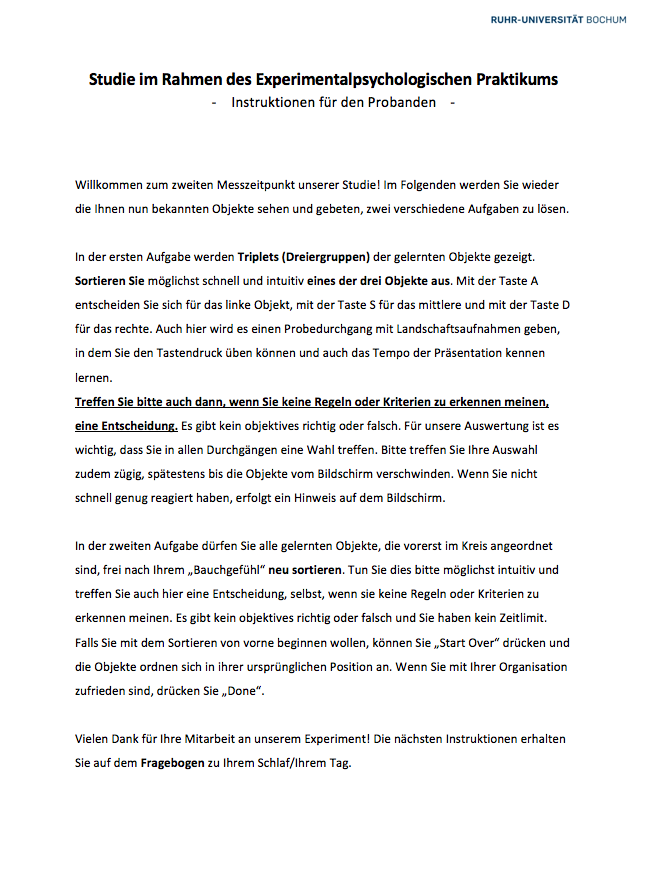
\includegraphics{Bilder/ProbT2.png}}
\end{figure}